\section{Introduction}

A \emph{digital twin} is a virtual system that runs alongside some physical process of interest and mimics its behaviour over time in response to user-provided interventions. 
%
This modelling approach promises to transform planning and decision-making across a breadth of fields, since it allows actions to be chosen with a fuller understanding of the range of possible outcomes that may result. %
Early research on digital twins has considered use-cases including aviation \cite{tuegel2011reengineering}, manufacturing \cite{lu2020digital}, healthcare \cite{corral2020digital,coorey2022health}, civil engineering \cite{sacks2020construction}, climate modelling \cite{bauer2021digital}, and agriculture \cite{jans2020digital}.
For a comprehensive overview of this emerging technology, we refer the reader to \cite{barricelli2019survey,jones2020characterising,niederer2021scaling}.

Many applications of digital twins are considered safety-critical, which means the cost of deploying an inaccurate twin to production is potentially very high.
%
As such, methodology for assessing the performance of a twin before its deployment is essential for the safe, widespread adoption of digital twins in practice \cite{niederer2021scaling}.
In this work, we consider the problem of assessing twin accuracy and propose a concrete, theoretically grounded, and general-purpose methodology to this end.
We focus specifically on the use of statistical methods that leverage data obtained from the real-world process that the twin is designed to model.
Such strategies are increasingly viable for many applications as datasets grow larger, and offer the promise of lower overheads compared with alternative strategies that rely for instance on domain expertise.

A principal design objective for digital twins is to improve decision-making, with much emphasis placed on their ability to reveal choices of actions that are expected to produce some desirable outcome in the real world \cite{barricelli2019survey,jones2020characterising,niederer2021scaling}.
We therefore adopt the position that, to be considered ``accurate'', a twin must capture the range of outcomes that \emph{would} occur when certain actions or interventions are applied to the real-world process of interest in a controlled way. %
%
Accordingly, we formulate twin assessment as a problem of \emph{causal inference} \cite{rubin1974estimating,rubin2005causal,pearl2009causality,hernan2020causal}, which offers a particularly suitable framework for reasoning about interventional behaviour of this kind.

The primary reason for assessing the accuracy of a twin is to determine its reliability and robustness.
It is therefore desirable for any assessment procedure itself to be reliable and robust, and for any conclusions it draws about the twin to be highly trustworthy.
%
%
As such, our goal in this paper is to obtain a methodology that is always \emph{sound}, even possibly at the expense of being conservative: we prefer not to draw any conclusion about the accuracy of the twin at all than to draw some conclusion that is potentially misleading.
To this end, we rely on minimal assumptions about the twin and the real-world process of interest.
In addition to improving robustness, this also means our resulting methodology is highly general, and so may be applied to a wide variety of twins across application domains.

%

%
%
%
%


%
%
%
%
%
%

\paragraph{Contribution}

Our contribution has the following components:
\begin{itemize}
    \item We show that if interventional information is sought from a twin, then it is not possible to use observational data to \emph{certify} that the twin is accurate unless strong and often tenuous assumptions are made about the data-generating process, such as that the data are free of unmeasured confounding.
    %
    %
    To avoid these assumptions, we advocate for an assessment paradigm instead based on \emph{falsification}: we aim to find specific examples of where the twin is \emph{not} accurate, rather than trying to quantify its overall accuracy in a holistic sense. %
    %
    \item We propose a general-purpose statistical testing procedure for falsifying a twin that relies on only the assumption of an independent and identically distributed (i.i.d.)\ dataset of observational trajectories.
    In particular, the procedure does not require modelling the dynamics of the real-world process or any internal implementation details of the twin, and remains sound in the presence of arbitrary unmeasured confounding. %
    Key to our approach is a novel longitudinal form of Manski's classical bounds \cite{manski} from the causal inference literature that may also be of interest in other contexts (see Section \ref{sec:causal-bounds}).
    \item We demonstrate the effectiveness of our procedure through a large-scale, real-world case study in which we use the MIMIC-III ICU dataset \cite{mimic} to assess the Pulse Physiology Engine \cite{pulse}, a high-fidelity, open-source model for human physiology simulation.
\end{itemize}

\paragraph{Related work}

%
Various high-level guidelines and workflows have been proposed for the assessment of digital twins in the literature to-date \cite{grieves2017digital,khan2018digital,corral2020digital,kochunas2021digital,niederer2021scaling,dahmen2022verification}, as well as in the field of computational science more broadly \cite{roy2011comprehensive,niederer2021scaling}. %
In some cases, these guidelines have been codified as standards: for example, the ASME V\&V40 Standard \cite{amse2018assessing} provides a risk-based framework for assessing the credibility of a model from a variety of factors that include source code quality and the mathematical form of the model \cite{galappaththige2022credibility}.
%
However, a significant gap still exists between these guidelines and a practical implementation that could be deployed for real twins, and the need for a rigorous lower-level framework to enable the systematic assessment of twins has been noted in this literature \cite{corral2020digital,niederer2021scaling,kapteyn2021probabilistic,masison2021modular}.
We contribute towards this effort by describing a precise statistical methodology for twin assessment that can be readily implemented in practice, and which is accompanied by theoretical guarantees of robustness that hold under minimal assumptions.
%

In addition, a variety of concrete assessment procedures have been applied to certain specific digital twin models in the literature.
For example, the Pulse Physiology Engine \cite{pulse}, which we consider in our empirical case study, as well as the related BioGears \cite{sepsis-modelling,biogears} were both assessed by comparing their outputs with ad hoc values based either on available medical literature or the opinions of subject matter experts.
Other twins have been assessed by comparing their outputs with real-world data through a variety of bespoke numerical schemes \cite{larrabide2012fast,hemmler2019patient,DT-patient,jans2020digital,galappaththige2022credibility}.
In contrast, our paper proposes a general-purpose statistical procedure for assessing twins that may be applied generically across many applications and architectures. %
To the best of our knowledge, our paper is also the first to identify the need for a causal approach to twin assessment and the pitfalls that arise when causal considerations are not properly accounted for.

%

\paragraph{Outline}

%
%
%
%

In Section \ref{sec:causal-formulation} we introduce precise causal models for the twin and the real-world process.
In Section \ref{sec:data-driven-twin-assessment}, we distinguish between certification and falsification assessment procedures, showing that certification is in general unsound and advocating for falsification as a more robust strategy.
%
In Section \ref{sec:causal-bounds}, we introduce and analyse a novel causal bound that in Section \ref{sec:hypotheses-from-causal-bounds} provides the basis for a hypothesis testing procedure for twin falsification with exact, finite-sample guarantees of validity under only the assumption of i.i.d.\ observational data.
%
Section \ref{sec:case-study} contains the results of our empirical case study. %
%
%
%

%

\section{Causal formulation} \label{sec:causal-formulation}

Here we provide causal models for the twin and the corresponding real-world process that the twin is designed to simulate.
We do so in the language of \emph{potential outcomes} \cite{rubin1974estimating,rubin2005causal}, although we note that we could have used the alternative framework of directed acyclic graphs and structural causal models \cite{pearl2009causality} (see also \cite{imbens2020potential} for a comparison of the two).
%

\subsection{The real-world process}

We assume the real-world process operates over a fixed time horizon $\T \in \{1, 2, \ldots\}$.
This simplifies our presentation in what follows, and it is straightforward to generalise our methodology to variable length time horizons if needed.
For each $\tx \in \{0, \ldots, \T\}$, we assume the process gives rise to a \emph{observation} at time $\tx$, which takes values in some real-valued space $\Xspace_\tx \coloneqq \R^{\Xspacedim_\tx}$.
%
We also assume that the process can be influenced by some \emph{action} taken at each time $\tx \in \{1, \ldots, \T\}$.
We denote the space of actions available at time $\tx$ by $\Aspace_\tx$, which in this work we assume is always finite.
For example, in a robotics context, the observations may consist of all the readings of all the sensors of the robot, and the actions may consist of commands that can be input by an external user.
In a medical context, the observations may consist of the vital signs of a patient, and the actions may consist of possible treatments or interventions.
To streamline notation, we will index these spaces using vector notation, so that e.g.\ $\Aspace_{1:\tx}$ denotes the cartesian product $\Aspace_1 \times \cdots \times \Aspace_\tx$, and $\ax_{1:\tx} \in \Aspace_{1:\tx}$ is a choice of $\ax_1 \in \Aspace_1, \ldots, \ax_\tx \in \Aspace_\tx$.

We model the dynamics of the real-world process via the longitudinal potential outcomes framework proposed by Robins \cite{robins1986new}, which imposes only a weak temporal structure on the underlying phenomena of interest and so may be applied across a wide range of applications in practice.
In particular, for each $\ax_{1:\T} \in \Aspace_{1:\T}$, we posit the existence of random variables or \emph{potential outcomes} $\X_0, \X_1(\ax_1), \ldots, \X_\T(\ax_{1:\T})$, where $\X_\tx(\ax_{1:\tx})$ takes values in $\Xspace_\tx$.
We will denote this sequence more concisely as $\X_{0:\T}(\ax_{1:\T})$.
%
Intuitively, $\X_0$ represents data available before the first action, while $\X_{1:\T}(\ax_{1:\T})$ represents the sequence of real-world outcomes that \emph{would} occur if actions $\ax_{1:\T}$ were taken successively.
These quantities are therefore of fundamental interest for planning a course of actions to achieve some desired result.

%

As random variables, each $\X_{\tx}(\ax_{1:\tx})$ may depend on additional randomness that is not explicitly modelled, and so in particular may be influenced by all the previous potential outcomes $\X_{0:\tx-1}(\ax_{1:\tx-1})$, and possibly other random quantities.
This models a process whose initial state is determined by external factors, such as when a patient from some population first presents at a hospital, and where the process then evolves according both to specific actions chosen from $\Aspace_{1:\T}$ as well as additional external factors.
It is clear that this structure applies to a wide range of phenomena occurring in practice.

%


\subsection{The digital twin}

We think of the twin as a computational device that, when executed, outputs a sequence of values intended to simulate a possible future trajectory of the real-world process when certain actions in $\Aspace_{1:\T}$ are chosen, conditional on some initial data in $\Xspace_0$.
We allow the twin to make use of an internal random number generator to produce outputs that vary stochastically even under fixed inputs (although our framework encompasses twins that evolve deterministically also).
By executing the twin repeatedly, a user may therefore estimate the range of behaviours that the real-world process may exhibit under different action sequences, which can in turn be used to guide planning and decision-making downstream.

Precisely, we model the output the twin would produce at timestep $\tx \in \{1, \ldots, \T\}$ after receiving initialisation $\xx_0 \in \Xspace_0$ and successive inputs $\ax_{1:\tx} \in \Aspace_{1:\tx}$ as the quantity $\twinfunction_\tx(\xx_0, \ax_{1:\tx}, \twinnoise_{1:\tx})$, where $\twinfunction_\tx$ is a measurable function taking values in $\Xspace_{\tx}$, and each $\twinnoise_\sx$ is some (possibly vector-valued) random variable.
We will denote $\Xt_{\tx}(\xx_0, \ax_{1:\tx}) \coloneqq \twinfunction_\tx(\xx_0, \ax_{1:\tx}, \twinnoise_{1:\tx})$, which we also refer to as a potential outcome.
%
%
A full twin trajectory therefore consists of $\Xt_1(\xx_0, \ax_1), \ldots, \Xt_\T(\xx_0, \ax_{1:\T})$, which we write more compactly by $\Xt_{1:\T}(\xx_0, \ax_{1:\T})$.
%
Conceptually, $\twinfunction_1, \ldots, \twinfunction_\T$ constitute the program that executes inside the twin, and $\twinnoise_{1:\T}$ may be thought of as the collection of all outputs of the internal random number generator that the twin uses.
%
We assume these random numbers $\twinnoise_{1:\T}$ and the real-world outcomes $(\X_{0:\T}(\ax_{1:\T}) : \ax_{1:\T} \in \Aspace_{1:\T})$ are independent, which is mild in practice.
We also assume that repeated executions of the twin give rise to i.i.d.\ copies of $\twinnoise_{1:\T}$.
This means that, given fixed inputs $\xx_0$ and $\ax_{1:\T}$, repeated executions of the twin produce i.i.d.\ copies of $\Xt_{1:\T}(\xx_0, \ax_{1:\T})$.
Otherwise, we make no assumptions about the precise form of either the $\twinfunction_\tx$ or the $\twinnoise_\tx$, which allows our model to encompass a wide variety of possible twin implementations.


\paragraph{Correctness}

%
%
We assume the twin has been designed to be correct in the following sense:

%


\begin{definition}[Correctness] \label{eq:interventional-correctness}
    The twin is \emph{interventionally correct} if, for $\Law[\X_0]$-almost all $\xx_0 \in \Xspace_0$ and $\ax_{1:\T} \in \Aspace_{1:\T}$, the distribution of $\Xt_{1:\T}(\xx_0, {\ax}_{1:\T})$ is equal\footnote{More generally we could allow for inequality up to some specified tolerance level. However, our stricter condition here is simpler, and suffices to convey the main ideas in what follows.} to the conditional distribution of $\X_{1:\T}(\ax_{1:\T})$ given $\X_0 = \xx_0$.
    %
    %
\end{definition}


Operationally, if this holds, then by repeatedly executing the twin and applying Monte Carlo techniques, it is possible to approximate arbitrarily well the conditional distribution of the future of the real-world process under each possible choice of action sequence.
The same can also be shown to hold when each action at each time $\tx$ is chosen dynamically on the basis of previous observations in $\Xspace_{0:\tx}$. %
As a result, an interventionally correct twin may be used for \emph{planning}, or in other words may be used to select a policy for choosing actions that will yield a desirable distribution over observations at each step.
%

We emphasise that interventional correctness does not mean the twin will accurately predict the behaviour of any \emph{specific} trajectory of the real-world process in an almost sure sense (unless the real-world process is deterministic), but only the distribution of outcomes that will be observed over repeated independent trajectories.
However, this is sufficient for many applications, and appears to be the strongest guarantee possible when dealing with real-world phenomena whose underlying behaviour is stochastic.

Definition \ref{eq:interventional-correctness} introduces some technical difficulties that arise in the general case when conditioning on events with probability zero (e.g.\ $\{\X_0 = \xx_0\}$ if $\X_0$ is continuous).
In what follows, it is more convenient to consider an unconditional formulation of interventional correctness.
This is supplied by the following result, which considers the behaviour of the twin when it is initialised with the (random) value of $\X_0$ taken from the real-world process, rather than with a fixed choice of $\xx_0$.
See Section \ref{sec:unconditional-interventional-correctness-proof} of the \AppendixName for a proof.

%
%
%
%
%
%
%
%
%
%
%
%

\begin{proposition} \label{prop:interventional-correctness-alternative-characterisation}
    The twin is interventionally correct if and only if, for all choices of $\ax_{1:\T} \in \Aspace_{1:\T}$, the distribution of $(\X_0, \Xt_{1:\T}(\X_0, \ax_{1:\T}))$ is equal to the distribution of $\X_{0:\T}(\ax_{1:\T})$.
\end{proposition}


%
%
%
%
%
%

%
%
%

\paragraph{Online prediction}

Our model here represents a twin at time $\tx = 0$ making predictions about all future timesteps $\tx \in \{1, \ldots, \T\}$ under different choices of inputs $\ax_{1:\T}$.
In practice, many twins are designed to receive new information at each timestep in an online fashion and update their predictions for subsequent timesteps accordingly \cite{grieves2017digital,niederer2021scaling}.
%
Various notions of correctness can be devised for this online setting.
We describe two possibilities in Section \ref{sec:online-prediction} of the \AppendixName, and show that these notions of correctness essentially reduce to Definition \ref{eq:interventional-correctness}, which motivates our focus on that notion in what follows.
%
%

\section{Data-driven twin assessment} \label{sec:data-driven-twin-assessment}

We now consider how to assess the accuracy of a twin.
There are many conceivable methods for doing this, including static analysis of the twin's source code and the solicitation of domain expertise, and in practice it seems most robust to use a combination of different techniques rather than relying on any single one \cite{amse2018assessing,niederer2021scaling,galappaththige2022credibility}.
However, in this paper, we focus on what we will call \emph{data-driven assessment}, which we see as an important component of a larger assessment pipeline. %
That is, we consider the use of statistical methods that rely solely on data obtained from the real-world process and trajectories simulated by the twin.
%
%
%
%
%
%
%
%
We show in this section that, without further assumptions, it is not possible to obtain a data-driven assessment procedure that can \emph{certify} that a twin is interventionally correct.
%
We instead propose a strategy based on \emph{falsifying} the twin, which we develop into a concrete statistical testing procedure in later sections.

%

%


\subsection{Certification is unsound in general}

\paragraph{Data model}

We assume access to a dataset of trajectories obtained by observing the interaction of some behavioural agents with the real-world process.
We model each trajectory as follows.
First, we represent the action chosen by the agent at time $\tx \in \{1, \ldots, \T\}$ as an $\Aspace_\tx$-valued random variable $\A_\tx$.
We then obtain a trajectory in our dataset by recording at each step the action $\A_\tx$ chosen and the observation $\X_\tx(\A_{1:\tx})$ corresponding to this choice of action.
%
As a result, each observed trajectory has the following form:
\begin{equation} \label{eq:observed-data-trajectory}
    \X_0, \A_1, \X_1(\A_1), \ldots, \A_\T, \X_\T(\A_{1:\T}).
\end{equation}
This corresponds to the standard \emph{consistency} assumption in causal inference \cite{hernan2020causal}, and intuitively means that the potential outcome $\X_\tx(\ax_{1:\tx})$ is observed in the data when the agent actually chose $\A_{1:\tx} = \ax_{1:\tx}$.
%
%
We model our full dataset as a set of i.i.d.\ copies of \eqref{eq:observed-data-trajectory}. %

%
%
%

%
\paragraph{Certification strategies}
%

%
A natural high-level strategy for twin assessment has the following structure.
First, some hypothesis $\Hyp$ is chosen with the following property:
%
 \begin{equation} \label{eq:verification-hypothesis-property}
    \text{If $\Hyp$ is true, then the twin is interventionally correct.}\footnote{More generally, and in practice more typically, we could consider a family of hypotheses that each imply correctness up to some tolerance level. However, \eqref{eq:verification-hypothesis-property} suffices for our exposition here.}
\end{equation}
%
Then data is used to try to show $\Hyp$ is true, perhaps up to some level of confidence. %
If successful, it follows by construction that the twin is interventionally correct.
Assessment procedures designed to \emph{certify} the twin in this way are appealing because they promise a strong guarantee of accuracy for certified twins. %
%
Unfortunately, the following foundational result from the causal inference literature (often referred to as the \emph{fundamental problem of causal inference} \cite{holland1986statistics}) means that data-driven certification procedures of this kind are in general unsound, as we explain next.
For completeness, Section \ref{sec:non-identifiability-result-proof-supp} of the \AppendixName includes a self-contained proof of this result in our notation.

%

%

%
%
%

\begin{theorem} \label{prop:nonidentifiability}
    %
    If $\Prob(\A_{1:\T} \neq \ax_{1:\T}) > 0$, then the distribution of $\X_{0:\T}(\ax_{1:\T})$ is not uniquely identified by the distribution of the data in \eqref{eq:observed-data-trajectory} without further assumptions.
\end{theorem}

%
%
%
%
%
%
%
%

Since the distribution of the data encodes the information that would be contained in an infinitely large dataset of trajectories, Theorem \ref{prop:nonidentifiability} imposes a fundamental limit on what can be learned about the distribution of $\X_{0:\T}(\ax_{1:\T})$ from the data we have assumed.
%
It follows that if $\Hyp$ is any hypothesis satisfying \eqref{eq:verification-hypothesis-property}, then $\Hyp$ cannot be determined to be true from even an infinitely large dataset.
This is because, if we could do so, then we could also determine the distribution of $\X_{0:\T}(\ax_{1:\T})$, since by Proposition \ref{prop:interventional-correctness-alternative-characterisation} this would be equal to the distribution of $(\X_0, \Xt_{\T}(\X_0, \ax_{1:\T}))$.
In other words, we cannot use the data alone to certify that the twin is interventionally correct.


\subsection{The assumption of no unmeasured confounding} \label{sec:no-unmeasured-confounding-assumption}

Theorem \ref{prop:nonidentifiability} is true in the general case, when no additional assumptions about the data-generating process are made.
One way forward is therefore to introduce assumptions under which the distribution of $\X_{0:\T}(\ax_{1:\T})$ \emph{can} be identified.
This would mean it is possible to certify that the twin is interventionally correct, since, at least in principle, we could simply check whether this matches the distribution of $(\X_0, \Xt_{1:\T}(\X_{0}, \ax_{1:\T}))$ produced by the twin.

The most common such assumption in the causal inference literature is that the data are free of \emph{unmeasured confounding}.
Informally, this holds when each action $\A_\tx$ is chosen by the behavioural agent solely on the basis of the information available at time $\tx$ that is actually recorded in the dataset, namely $\X_{0}, \A_1, \X_1(\A_1), \ldots, \A_{\tx-1}, \X_{\tx-1}(\A_{1:\tx-1})$, as well as possibly some additional randomness that is independent of the real-world process, such as the outcome of a coin toss.\footnote{This can be made precise via the \emph{sequential randomisation assumption} (also known as \emph{sequential ignorability}) introduced by Robins \cite{robins1986new}. Chapter 5 of \cite{tsiatis2019dynamic} provides an overview of this.}
%
Unobserved confounding is present whenever this does not hold, i.e.\ whenever some unmeasured factor simultaneously influences both the agent's choice of action and the observation produced by the real-world process.
%

It is reasonable to assume that the data are unconfounded in certain contexts.
For example, in certain situations it may be possible to gather data in a way that specifically guarantees there is no confounding.
Randomised controlled trials, which ensure that each $\A_\tx$ is chosen via a carefully designed randomisation procedure \cite{lavori2004dynamic,murphy2005experimental}, constitute a widespread example of this approach.
Likewise, it is possible to show\footnote{See Section \ref{eq:deterministic-potential-outcomes-are-unconfounded} of the \AppendixName for a proof.} that the data are unconfounded if each $\X_\tx(\ax_{1:\tx})$ is a deterministic function of $\X_{0:\tx-1}(\ax_{1:\tx-1})$ and $\ax_{\tx}$, which may be reasonable to assume for example in certain low-level physics or engineering contexts.
However, for stochastic phenomena and for typical datasets, it is widely acknowledged that the assumption of no unmeasured confounding will rarely hold, and so assessment procedures based on this assumption may yield unreliable results in practice \cite{murphy2003optimal,tsiatis2019dynamic}.
Section \ref{sec:motivating-example} of the \AppendixName illustrates this concretely with a toy scenario.
%
%

%
%


\subsection{General-purpose assessment via falsification}

Our goal is to obtain an assessment methodology that is general-purpose, and as such we would like to avoid introducing assumptions such as unconfoundedness that do not hold in general.
%
To achieve this, borrowing philosophically from Popper \cite{popper2005logic}, we propose a strategy that replaces the goal of verifying the interventional correctness of the twin with that of \emph{falsifying} it.
Specifically, we consider hypotheses $\Hyp$ with the dual property to \eqref{eq:verification-hypothesis-property}, namely:
\begin{equation} \label{eq:falsification-hypothesis-property}
    \text{If the twin is interventionally correct, then $\Hyp$ is true.}
\end{equation}
We will then try to show that each such $\Hyp$ is \emph{false}.
%
Whenever we are successful, we will thereby have gained some knowledge about a failure mode of the twin, since by construction the twin can only be correct if $\Hyp$ is true.
In effect, each $\Hyp$ we falsify will constitute a \emph{reason} that the twin is not correct, and may suggest concrete improvements to its design, or may identify cases where its output should not be trusted.

Importantly, unlike for \eqref{eq:verification-hypothesis-property}, Theorem \ref{prop:nonidentifiability} does not preclude the possibility of data-driven assessment procedures based on \eqref{eq:falsification-hypothesis-property}.
As we show below, there do exist hypotheses $\Hyp$ satisfying \eqref{eq:falsification-hypothesis-property} that can in principle be determined to be false from the data alone without additional assumptions.
In this sense, falsification provides a means for \emph{sound} data-driven twin assessment, %
whose results can be relied upon across a wide range of circumstances.
On the other hand, falsification approaches cannot provide a \emph{complete} guarantee about the accuracy of a twin: even if we fail to falsify many $\Hyp$ satisfying \eqref{eq:falsification-hypothesis-property}, we cannot then infer that the twin is correct.
As such, in situations where (for example) it is reasonable to believe that the data are in fact unconfounded, it may be desirable to use this assumption to obtain additional information about the twin than is possible from falsification alone.
%


%
%
%
%
%
%
%
%
%

%
%
%
%
%
%
%
%


%
%
%
%


%

%

%
%



%



\section{Causal bounds} \label{sec:causal-bounds}

We now describe a novel longitudinal variant of Manski's classical bounds \cite{manski} from the causal inference literature.
Intuitively, this result bounds the expected outcome output by any interventionally correct twin.
In the next section, we use this result to define hypotheses $\Hyp$ with the desired property \eqref{eq:falsification-hypothesis-property}, which then yields a procedure for falsifying twins via hypothesis testing techniques.
%
%
%
%
%
%
%
We state the result before providing intuition below.
A proof is given in Section \ref{sec:causal-bounds-proofs} of the \AppendixName.

\begin{theorem} \label{thm:causal-bounds}
    Suppose $(\Y(\ax_{1:\tx}) : \ax_{1:\tx} \in \Aspace_{1:\tx})$ are real-valued potential outcomes, and that for some $\tx \in \{1, \ldots, \T\}$, $\ax_{1:\tx} \in \Aspace_{1:\tx}$, measurable $\B_{0:\tx} \subseteq \Xspace_{0:\tx}$, and $\ylo, \yup \in \R$ we have
%
\noindent
%
%
%
%
%
%
%
%
%
%
%
%
    \begin{gather}
        \Prob(\X_{0:\tx}(\ax_{1:\tx}) \in \B_{0:\tx}) > 0 \label{eq:B-positivity-assumption} \\
        \Prob(\ylo \leq \Y(\ax_{1:\tx}) \leq \yup \mid \X_{0:\tx}(\ax_{1:\tx}) \in \B_{0:\tx}) = 1.  \label{eq:Y-boundedness-assumption}
    \end{gather}
    \noindent Then it holds that
    \begin{equation} \label{eq:causal-bounds-fully-written}
         \E[\Ylo \mid \X_{0:\N}(\A_{1:\N}) \in \B_{0:\N}]
        \leq \E[\Y(\ax_{1:\tx}) \mid \X_{0:\tx}(\ax_{1:\tx}) \in \B_{0:\tx}]
        \leq  \E[\Yup \mid \X_{0:\N}(\A_{1:\N}) \in \B_{0:\N}] 
    \end{equation}
    %
    where we define $\N \coloneqq \max \{0 \leq \sx \leq \tx \mid \A_{1:\sx} = \ax_{1:\sx}\}$, and similarly
    \begin{align*}
        \Ylo \coloneqq \ind(\A_{1:\tx} &= \ax_{1:\tx}) \, \Y(\A_{1:\tx}) + \ind(\A_{1:\tx} \neq \ax_{1:\tx}) \, \ylo,\\
        \Yup \coloneqq \ind(\A_{1:\tx} &= \ax_{1:\tx}) \, \Y(\A_{1:\tx}) + \ind(\A_{1:\tx} \neq \ax_{1:\tx}) \, \yup.
    \end{align*}

    %
    
    %
    %
    %
    %
    %
    %
    %
    %
    %
\end{theorem}

\noindent
We will write the terms in \eqref{eq:causal-bounds-fully-written} as $\Qlo$, $\Q$, and $\Qup$ respectively, so we have $\Qlo \leq \Q \leq \Qup$.

\paragraph{Intuition}

Here $\Y(\ax_{1:\tx})$ may be thought of as some quantitative outcome of interest.
For example, in a medical context, $\Y(\ax_{1:\tx})$ might represent the heart rate of a patient at time $\tx$ after receiving some treatments $\ax_{1:\tx}$.
When defining our hypotheses below, we consider the specific form $\Y(\ax_{1:\tx}) \coloneqq \fx(\X_{0:\tx}(\ax_{1:\tx}))$, where $\fx : \Xspace_{0:\tx} \to \R$ is some scalar function.
The value $\Q$ is then simply the (conditional) average behaviour of this outcome.
By Theorem \ref{prop:nonidentifiability}, $\Q$ is in general not identified by the data since it depends on $\X_{0:\tx}(\ax_{1:\tx})$.
%
%
%
On the other hand, both $\Qlo$ and $\Qup$ \emph{are} identifiable, since the relevant random variables $\Ylo$, $\Yup$, $\N$, and $\X_{0:\N}(\A_{1:\N})$ can all be expressed as functions of the observed data $\X_{0:\tx}(\A_{1:\tx})$ and $\A_{1:\tx}$.
In this way, Theorem \ref{thm:causal-bounds} bounds the behaviour of a non-identifiable quantity in terms of identifiable ones.
At a high level, this is achieved by replacing $\Y(\ax_{1:\tx})$, whose value is only observed when $\A_{1:\tx} = \ax_{1:\tx}$, with $\Ylo$ and $\Yup$, which are equal to $\Y(\ax_{1:\tx})$ when its value is observed (i.e.\ when $\A_{1:\tx} = \ax_{1:\tx}$), and which fall back to the worst-case values of $\ylo$ and $\yup$ otherwise.
%
We emphasise that Theorem \ref{thm:causal-bounds} does not require any additional causal assumptions, and in particular remains true under arbitrary unmeasured confounding.

%
%

%

% \begin{importantresultwithtitle}[title=Related results]\noindent
\paragraph{Related results}
Theorem \ref{thm:causal-bounds} is a longitudinal generalisation of Manski's classical bounds from \cite{manski}.\footnote{We make this relationship precise in Section \ref{sec:continuous-initial-covariates-supplement} of the \AppendixName.}
In the structural causal modelling framework \cite{pearl2009causality}, a related bound was recently given by Zhang \& Bareinboim as Corollary 1 in \cite{bareinboim}.
However, their result involves a complicated ratio of unknown quantities that makes estimation of their bounds difficult, since it is not obvious how to obtain an unbiased estimator for the ratio term.
In contrast, our proposed causal bounds are considerably simpler, since both $\Qlo$ and $\Qup$ here are expressed as (conditional) expectations. 
This makes their unbiased estimation straightforward, which we use to obtain exact confidence intervals for both terms in Section \ref{sec:statistical-methodology}.
% \end{importantresultwithtitle}

%

%
%



\paragraph{Tightness of bounds}

Straightforward manipulations yield the following:
\[
    \frac{\Qup - \Qlo}{\yup - \ylo} = 1 - \Prob(\A_{1:\tx} = \ax_{1:\tx} \mid \X_{0:\N}(\A_{1:\N}) \in \B_{0:\N}).
\]
Here the left-hand side quantifies the \emph{tightness} of the bounds $[\Qlo, \Qup]$ relative to the worst-case bounds $[\ylo, \yup]$ that are trivially implied by \eqref{eq:Y-boundedness-assumption}, with smaller values meaning tighter bounds.
In this way, the tightness of the bounds is determined by the value of $\Prob(\A_{1:\tx} = \ax_{1:\tx} \mid \X_{0:\N}(\A_{1:\N}) \in \B_{0:\N})$, which is closely related to the classical \emph{propensity score} in the causal inference literature \cite{rosenbaum1983central}. %
Intuitively, as $\Prob(\A_{1:\tx} = \ax_{1:\tx} \mid \X_{0:\N}(\A_{1:\N}) \in \B_{0:\N})$ grows larger, $\Y(\ax_{1:\tx}) = \Y(\A_{1:\tx})$ holds on the event $\{\X_{0:\N}(\A_{1:\N}) \in \B_{0:\N}\}$ with higher probability, so that the effect of unmeasured confounding on the overall expectation $\Q = \E[\Y(\ax_{1:\tx}) \mid \X_{0:\tx}(\ax_{1:\tx}) \in \B_{0:\tx}]$ is reduced, and  $\Q$ may be bounded more tightly.
%

%



%




%
%
%
%
%
%
%
%
%
%

\paragraph{Sharpness of bounds}

%
%
%
The following result shows that Theorem \ref{thm:causal-bounds-supp} cannot be improved without further assumptions. 
Intuitively, the result states that there always exists \emph{some} potential outcomes family which leads to the same observational data as our model, but which attains the worst-case bounds $\Qlo$ or $\Qup$.
Therefore, we cannot rule out the possibility that our model achieves $\Qlo$ or $\Qup$ from the observational data alone.
%
%
%

\begin{proposition} \label{prop:sharpness-of-bounds}
    Under the same setup as in Theorem \ref{thm:causal-bounds}, there always exists potential outcomes $(\tilde{\X}_{0:\T}(\ax_{1:\T}'), \tilde{\Y}(\ax_{1:\tx}') : \ax_{1:\T}' \in \Aspace_{1:\T})$ also satisfying \eqref{eq:Y-boundedness-assumption} (mutatis mutandis) with 
    $$(\tilde{\X}_{0:\T}(\A_{1:\T}), \tilde{\Y}(\A_{1:\tx}), \A_{1:\T}) \eqas (\X_{0:\T}(\A_{1:\T}), \Y(\A_{1:\tx}), \A_{1:\T})$$ 
    but for which $$\E[\tilde{\Y}(\ax_{1:\tx}) \mid \tilde{\X}_{0:\tx}(\ax_{1:\tx}) \in \B_{0:\tx}] = \Qlo.$$
    The corresponding statement is also true for $\Qup$.
\end{proposition}

\paragraph{Pointwise conditional bounds}

%

%
In some cases, it may be desirable to obtain bounds on the alternative quantity $\E[\Y(\ax_{1:\tx}) \mid \X_{0:\tx}(\ax_{1:\tx})]$, i.e.\ conditional on the \emph{value} of $\X_{0:\tx}(\ax_{1:\tx})$ rather than on the event $\{\X_{0:\tx}(\ax_{1:\tx}) \in \B_{0:\tx}\}$.
%
To achieve this, it is natural to generalise our assumption \eqref{eq:Y-boundedness-assumption} by supposing we have measurable functions $\ylo, \yup : \Xspace_{0:\tx} \to \R$ such that
\begin{equation} \label{eq:worst-case-behaviour-functional-assumption}
    \ylo(\X_{0:\tx}(\ax_{1:\tx})) \leq \Y(\ax_{1:\tx}) \leq \yup(\X_{0:\tx}(\ax_{1:\tx})) \qquad \qquad \text{almost surely.}
\end{equation}
When this holds, almost sure bounds on $\E[\Y(\ax_{1:\tx}) \mid \X_{0:\tx}(\ax_{1:\tx})]$ can be obtained directly from Theorem \ref{thm:causal-bounds} if $\X_{0:\tx}(\ax_{1:\tx})$ is discrete, or by a simple modification of the proof of Theorem \ref{thm:causal-bounds} if $\X_{1:\tx}(\ax_{1:\tx})$ is discrete (but $\X_0$ is possibly continuous), which recovers Manski's original bounds from \cite{manski} as a special case.
We discuss this further in Section \ref{sec:impossibility-of-bounds-for-continuous-data} of the \AppendixName.

However, somewhat surprisingly, if the distribution of $\X_{1:\tx}(\ax_{1:\tx})$ is not discrete, then we cannot obtain nontrivial bounds of this kind without further assumptions.
To make this precise, we will say that candidate bounds $\lo{\gx}, \up{\gx} : \Xspace_{0:\tx} \to \R$ are \emph{permissible} if
\begin{equation} \label{eq:glo-works-for-all-models}
    \lo{\gx}(\tilde{\X}_{0:\tx}(\ax_{1:\tx})) \leq \E[\tilde{\Y}(\ax_{1:\tx}) \mid \tilde{\X}_{0:\tx}(\ax_{1:\tx})] \leq \up{\gx}(\tilde{\X}_{0:\tx}(\ax_{1:\tx})) \qquad \qquad \text{almost surely}
\end{equation}
for all potential outcomes $(\tilde{\X}_{0:\T}(\ax_{1:\T}'), \tilde{\Y}(\ax_{1:\tx}'), \tilde{\A}_{1:\T} : \ax_{1:\T}' \in \Aspace_{1:\T})$ that also satisfy \eqref{eq:worst-case-behaviour-functional-assumption} (mutatis mutandis) with $\Law[\tilde{\X}_{0:\T}(\tilde{\A}_{1:\T}), \tilde{\A}_{1:\T}, \tilde{\Y}(\tilde{\A}_{1:\tx})] = \Law[\X_{0:\T}(\A_{1:\T}), \A_{1:\T}, \Y(\A_{1:\tx})]$.
Intuitively, this means that $\lo{\gx}$ and $\up{\gx}$ depend only on the information we have available, i.e.\ our assumed worst-case values and the observational distribution.
We then have the following:

%
%

%

%
%
%
%
%

\begin{theorem} \label{thm:no-causal-bounds-for-continuous-data}
    Suppose $\X_0$ is almost surely constant, $\Prob(\A_1 \neq \ax_1) > 0$, and for some $\sx \in \{1, \ldots, \tx\}$ we have $\Prob(\X_{\sx}(\A_{1:\sx}) = \xx_{\sx}) = 0$ for all $\xx_{\sx} \in \Xspace_{\sx}$.
    Then $\lo{\gx}, \up{\gx} : \Xspace_{0:\tx} \to \R$ are permissible bounds only if they are trivial, i.e.,
    \begin{align*}
        \lo{\gx}(\X_{0:\tx}(\ax_{1:\tx})) \leq \ylo(\X_{0:\tx}(\ax_{1:\tx})) \quad \textup{and} \quad \up{\gx}(\X_{0:\tx}(\ax_{1:\tx})) \geq \yup(\X_{0:\tx}(\ax_{1:\tx})) \quad \textup{almost surely.}
    \end{align*}
    % $\lo{\gx}(\X_{0:\tx}(\ax_{1:\tx})) \leq \ylo(\X_{0:\tx}(\ax_{1:\tx}))$ and $\up{\gx}(\X_{0:\tx}(\ax_{1:\tx})) \geq \yup(\X_{0:\tx}(\ax_{1:\tx}))$ almost surely.
    %
\end{theorem}

Here the assumption that $\X_0$ is constant essentially means we consider a special case of our model where there are no covariates available before the first action is taken, and serves mainly to simplify the proof.
We conjecture that Theorem \ref{thm:no-causal-bounds-for-continuous-data} holds more generally, provided the other assumptions are made conditional on $\X_0$ accordingly.
%
%
In any case, this result shows that general purpose bounds on $\E[\Y(\ax_{1:\tx}) \mid \X_{0:\tx}(\ax_{1:\tx})]$ are not forthcoming, and Theorem \ref{thm:causal-bounds} is the best we can hope for in general.
We show below that this result is nevertheless powerful enough to obtain useful information in practice.

%
%
%
%
%
%


\section{Falsification methodology} \label{sec:hypotheses-from-causal-bounds}

%

We now use Theorem \ref{thm:causal-bounds} to define a hypothesis testing methodology that can be used to falsify the twin.
We first define the hypotheses $\Hyp$ satisfying \eqref{eq:falsification-hypothesis-property} that we will consider, and then give a statistical procedure for testing these while controlling for type I error.
Our overall procedure does not rely on any further assumptions than we have already provided.

%

%


%

\subsection{Hypotheses derived from causal bounds}

Each hypothesis we test will depend on a specific choice of the following parameters:

\begin{multicols}{2}
    \begin{itemize}
        \item A timestep $\tx \in \{1, \ldots, \T\}$
        \item A measurable function $\fx : \Xspace_{0:\tx} \to \R$
    \end{itemize}
    \columnbreak
    \begin{itemize}
        \item A sequence of actions $\ax_{1:\tx} \in \Aspace_{1:\tx}$
        \item A sequence of subsets $B_{0:t} \subseteq \Xspace_{0:t}$. 
    \end{itemize}
\end{multicols}

%
%
%
\noindent
To streamline notation, in this section, we will consider these parameters to be fixed.
However, we emphasise that our construction can be instantiated for many different choices of these parameters, and indeed we will do so in our case study below.
We think of $\fx$ as expressing a specific outcome of interest at time $\tx$ in terms of the data we have assumed.
Accordingly, for each $\ax_{1:\tx}' \in \Aspace_{1:\tx}$, we define new potential outcomes
$\Y(\ax_{1:\tx}') \coloneqq \fx(\X_{0:\tx}(\ax_{1:\tx}'))$.
%
    %
%
%
For example, in a medical context, if $\X_{0:\tx}(\ax_{1:\tx}')$ represents a full patient history at time $\tx$ after treatments $\ax_{1:\tx}'$, then $\Y(\ax_{1:\tx}')$ might represent the patient's heart rate after these treatments. 
Likewise, $\B_{0:\tx}$ selects a subgroup of patients of interest, e.g.\ elderly patients whose blood pressure values were above some threshold at some timesteps before $\tx$.

%
%

%
%

%


%
%


\paragraph{Hypothesis definition}

The hypotheses we consider are based on the corresponding outcome produced by the twin when initialised at $\X_0$, which we define for $\ax_{1:\tx}' \in \Aspace_{1:\tx}$ as $\Yt(\ax_{1:\tx}') \coloneqq \fx(\X_0, \Xt_{1:\tx}(\X_0, \ax_{1:\tx}'))$.
Supposing it holds that
\begin{equation} \label{eq:B-twin-positivity-assumption}
    \Prob(\Xt_{1:\tx}(\X_0, \ax_{1:\tx}) \in \B_{1:\tx}) > 0,
\end{equation}
we may then define
%
$\Qt \coloneqq \E[\Yt(\ax_{1:\tx}) \mid \X_0 \in \B_0, \Xt_{1:\tx}(\X_0, \ax_{1:\tx}) \in \B_{1:\tx}]$, i.e.\
the analogue of $\Q$ for the twin.
By Proposition \ref{prop:interventional-correctness-alternative-characterisation}, if the twin is interventionally correct, then $\Qt = \Q$.
Theorem \ref{thm:causal-bounds} therefore implies that the following hypotheses have our desired property \eqref{eq:falsification-hypothesis-property}:
%
\begin{gather*}
\text{$\Hlo$: If \eqref{eq:B-positivity-assumption}, \eqref{eq:Y-boundedness-assumption}, and \eqref{eq:B-twin-positivity-assumption} hold, then $\Qt \geq \Qlo$} \\
\text{$\Hup$: If \eqref{eq:B-positivity-assumption}, \eqref{eq:Y-boundedness-assumption}, and \eqref{eq:B-twin-positivity-assumption} hold, then $\Qt \leq \Qup$.}
\end{gather*}
Moreover, $\Hlo$ and $\Hup$ can in principle be determined to be true or false from the information we have assumed available, since $\Qlo$ and $\Qup$ depend only on the observational data, and $\Qt$ can be estimated by generating trajectories from the twin.

%

%

%

%
%
%
%
%
%


%
%
%
%
%

%

%

%
%
%
%
%
%
%
%

\paragraph{Interpreting a falsification}

From a practical perspective, falsifying either $\Hlo$ or $\Hup$ leads to knowledge about a specific failure mode of the twin with various potential implications downstream.
For example, if $\Hlo$ is false (i.e.\ if $\Qt < \Qlo$), it follows that, among those trajectories for which $(\X_0, \Xt_{1:\tx}(\X_0, \ax_{1:\tx})) \in \B_{0:\tx}$, the corresponding value of $\Yt(\ax_{1:\tx})$ is on average too small. %
In light of this, a user might choose not to rely on outputs of the twin produced under these circumstances, while a developer seeking to improve the twin could focus their attention on the specific parts of its implementation that give rise to this behaviour.
We illustrate this concretely through our case study in Section \ref{sec:case-study}.

%

%

%
%
%
%

%

\subsection{Exact testing procedure} \label{sec:statistical-methodology}

%
We now describe a procedure for testing $\Hlo$ and $\Hup$ using a finite dataset that obtains exact control over type I error without relying on additional assumptions or asymptotic approximations.
We show in our case study below that this procedure is nevertheless powerful enough to obtain useful information about a twin in practice.

%

%
%
%

%

%

%

%

We focus here on obtaining a p-value for $\Hlo$ given a fixed choice of parameters $(\tx, \fx, \ax_{1:\tx}, \B_{0:\tx})$.
Our procedure for $\Hup$ is symmetrical, or may be regarded as a special case of testing $\Hlo$ by replacing $\fx$ with $-\fx$.
Multiple hypotheses may then be handled via standard techniques such as the Holm-Bonferroni \cite{holm1979simple} method (which we employ in our case study) or the Benjamini–Yekutieli \cite{benjamini2001control} procedure, both of which are valid without additional assumptions.
%
%
%

\paragraph{Datasets}

As above, we assume access to a finite dataset $\D$ of i.i.d.\ copies of \eqref{eq:observed-data-trajectory}.
We also assume access to a dataset $\Dt(\ax_{1:\tx})$ of i.i.d.\ copies of
\begin{equation} \label{eq:twin-trajecs}
    \X_0, \Xt_1(\X_0, \ax_1), \ldots, \Xt_\tx(\X_0, \ax_{1:\tx}).
\end{equation}
In practice, these copies can be obtained by initialising the twin with some value $\X_0$ taken from $\D$ without replacement and supplying inputs $\ax_{1:\tx}$.
If each $\X_0$ in $\D$ is used to initialise the twin at most once, then the resulting trajectories in $\Dt(\ax_{1:\tx})$ are guaranteed to be i.i.d., since we assumed in Section \ref{sec:causal-formulation} that the potential outcomes $\Xt_\tx(\xx_0, \ax_{1:\tx})$ produced by the twin are independent across runs.
We adopt this approach in our case study.

%

%
%

\paragraph{Antecedent conditions}

Observe that $\Hlo$ is false only if \eqref{eq:B-positivity-assumption}, \eqref{eq:Y-boundedness-assumption}, and \eqref{eq:B-twin-positivity-assumption} all hold.
We account for this in our testing procedure as follows.
First, \eqref{eq:Y-boundedness-assumption} immediately follows if 
%
\begin{equation} \label{eq:fx-boundedness-assumption}
    \ylo \leq \fx(\xx_{0:\tx}) \leq \yup \qquad \text{for all $\xx_{0:\tx} \in \B_{0:\tx}$.}
\end{equation}
This holds automatically in certain cases, such as when dealing with a binary outcome (e.g.\ patient survival), or otherwise can be enforced simply by clipping the value of $\fx$ to live within $[\ylo, \yup]$.
We describe a practical scheme for choosing $\fx$ in this way in Section \ref{sec:case-study}.

To account for \eqref{eq:B-positivity-assumption} and \eqref{eq:B-twin-positivity-assumption}, our first step in our testing process is simply to check whether there is some trajectory in $\D$ with $\A_{1:\tx} = \ax_{1:\tx}$ and $\X_{0:\tx}(\A_{1:\tx}) \in \B_{0:\tx}$, and some trajectory in $\Dt(\ax_{1:\tx})$ with $(\X_0, \Xt_{1:\tx}(\X_0, \ax_{1:\tx})) \in \B_{0:\tx}$.
If there are not, then we refuse to reject $\Hlo$ at any significance level; otherwise, we proceed to test $\Qt \geq \Qlo$ as described next.
%
%
%
It easily follows that there is zero probability we will reject $\Hlo$ if \eqref{eq:B-positivity-assumption} and \eqref{eq:B-twin-positivity-assumption} do not in fact hold, and so our overall type I error is controlled at the desired level.

%

%



\paragraph{Testing procedure}

%
%

To test $\Qt \geq \Qlo$, we begin by constructing a one-sided lower confidence interval for $\Qlo$, and a one-sided upper confidence interval for $\Qt$.
In detail, for each significance level $\alpha \in (0, 1)$, we obtain $\qlo{\alpha}$ and $\qt{\alpha}$ as functions of $\D$ and $\Dt(\ax_{1:\tx})$ such that
\begin{equation}
    \Prob(\Qlo \geq \qlo{\alpha}) \geq 1 - \frac{\alpha}{2} \qquad\,\, \Prob(\Qt \leq \qt{\alpha}) \geq 1 - \frac{\alpha}{2}. \label{eq:q-confidence-interval-new}
\end{equation}
%
%
%
%
We will also ensure that these are nested, i.e.\ $\qlo{\alpha} \leq \qlo{\alpha'}$ and $\qt{\alpha'} \leq \qt{\alpha}$ if $\alpha \leq \alpha'$.
%
%
We describe two methods for obtaining $\qlo{\alpha}$ and $\qt{\alpha}$ satisfying these conditions below.

From these confidence intervals, we obtain a test for the hypothesis $\Qt \geq \Qlo$ that rejects when $\qt{\alpha} < \qlo{\alpha}$.
A straightforward argument given in Section \ref{sec:hyp-testing-supplement} of the \AppendixName shows that this controls the type I error at the desired level $\alpha$.
%
Nestedness also yields a $p$-value obtained as the smallest value of $\alpha$ for which this test rejects, i.e.\
$\plo \coloneqq \inf\{\alpha \in (0, 1) \mid \text{$\qt{\alpha} < \qlo{\alpha}$}\}$,
%
%
%
%
or $1$ if the test does not reject at any level.
%

\paragraph{Confidence intervals}

We now consider how to obtain confidence intervals for $\Qlo$ and $\Qt$ satisfying the desired conditions above.
To this end, observe that both quantities are (conditional) expectations involving random variables that can be computed from $\D$ or $\Dt(\ax_{1:\tx})$.
This allows both to be estimated unbiasedly, which in turn can be used to derive confidence intervals via standard techniques.
For example, consider the subset of trajectories in $\Dt(\ax_{1:\tx})$ with $(\X_0, \Xt_{\tx}(\X_0, \ax_{1:\tx})) \in \B_{0:\tx}$.
For each such trajectory, we obtain a corresponding value of $\Yt(\ax_{1:\tx})$ that is i.i.d.\ and has expectation $\Qt$.
Similarly, for $\Qlo$, we extract the subset of trajectories in $\D$ for which $\X_{0:\N}(\A_{1:\N}) \in \B_{0:\N}$ holds. %
The values of $\Ylo$ obtained from each such trajectory are then i.i.d.\ and have expectation $\Qlo$.

At this point, our problem now reduces to that of constructing a confidence interval for the expectation of a random variable using i.i.d.\ copies of it.
Various techniques exist for this, and we consider two possibilities in our case study.
The first leverages the fact that $\Yt(\ax_{1:\tx})$ and $\Ylo$ are bounded in $[\ylo, \yup]$, which gives rise to $\qlo{\alpha}$ and $\qt{\alpha}$ via an application of Hoeffding's inequality.
This approach has the appealing property that \eqref{eq:q-confidence-interval-new} holds exactly, although often at the expense of conservativeness.
In practice, this could be mitigated by instead obtaining confidence intervals via (for example) the bootstrap \cite{efron1979bootstrap}, although at the expense of requiring (often mild) asymptotic assumptions.
%
Section \ref{sec:confidence-intervals-methodology-supplement} of the \AppendixName describes both methods in greater detail.
Our empirical results reported in the next section all use Hoeffding's inequality are hence exact, but we also provide some additional results obtained using bootstrapping in Section \ref{sec:boostrapping-details-supplement} of the \AppendixName.

%
%
%
%

%

%

%
%
%
%
%

%

%
%
%
%
%
%


%

%

%
%
%
%
%
%
%
%
%
%
%
%
%
%
%
%
%
%
%
%
%
%
%
%
%

%

%

%
%
%
%
%
%
%

\section{Case Study: Pulse Physiology Engine} \label{sec:case-study}

We applied our assessment methodology to the Pulse Physiology Engine \cite{pulse}, an open-source model for human physiology simulation.
Pulse simulates trajectories of various physiological metrics for patients with conditions like sepsis, COPD, and ARDS.
%
%
We describe the main steps of our experimental procedure and results below, with full details given in the Section \ref{sec:experiments-supplement} of the \AppendixName. 
%

\subsection{Experimental setup} \label{sec:experimental-setup}

\paragraph{Real-world data}

We utilized the MIMIC-III dataset \cite{mimic}, a comprehensive collection of longitudinal health data from critical care patients at the Beth Israel Deaconess Medical Center (2001-2012).
We focused on patients meeting the sepsis-3 criteria \cite{sepsis-criteria}, following the methodology of \cite{ai-clinician} for selecting these.
This yielded 11,677 sepsis patient trajectories.
We randomly selected 5\% of these (583 trajectories, denoted as $\D_0$) to use for choosing the parameters of our hypotheses via a sample splitting approach \cite{cox1975note}, with the remaining 95\% (11,094 trajectories, denoted as $\D$) reserved for the actual testing.

%

\paragraph{Observation and action spaces}

%
%

%

%


We considered hourly observations of each patient over the the first four hours of their ICU stay, i.e.\ $\T = 4$.
We defined the observation spaces $\Xspace_{0:\T}$ using a total of 17 features included in our extracted MIMIC trajectories for this time period, including static demographic quantities and patient vitals.
%
%
Following \cite{ai-clinician}, the actions we considered were the administration of intravenous fluids and vasopressors, which both play a primary role in the treatment of sepsis in clinical practice.
Since these are recorded in MIMIC as continuous doses, we discretised their values via the same procedure as \cite{ai-clinician}, obtaining finite action spaces $\Aspace_1 = \cdots = \Aspace_4$, each with $25$ distinct actions.

%
%
%



%
%
%
%
%
%
%
%

%

%
%
%


%
%


%

\paragraph{Hypothesis parameters} 

We defined a collection of hypothesis parameters $(\tx, \fx, \ax_{1:\tx}, \B_{0:\tx})$, each of which we then used to define an $\Hlo$ and $\Hup$ to test.
For this, we chose 14 different physiological quantities of interest to assess, including heart rate, skin temperature, and respiration rate (see Table \ref{tab:hypotheses_hoeffding_full} in the \AppendixName for a complete list).
For each of these, we selected combinations of $\tx$, $\ax_{1:\tx}$, and $\B_{0:\tx}$ observed for at least one patient trajectory in $\D_0$.
We took \(\ylo\) and \(\yup\) to be the .2 and .8 quantiles\footnote{We also investigated the sensitivity of our procedure to the choice of these quantiles and found it to be relatively stable (see Section \ref{sec:sensitity-analysis-appendix} of the \AppendixName).} of the same physiological quantity as recorded in $\D_0$, and   defined $\fx$ as the function that extracts this quantity from \(\Xspace_\tx\) and clips its value between \(\ylo\) and \(\yup\), so that \eqref{eq:fx-boundedness-assumption} holds.
We describe this procedure in full in Section \ref{sec:hypothesis-parameters-supplement} of the \AppendixName.
%
We obtained 721 unique parameter choices, leading to 1,442 total hypotheses.
%
%

%

%
%
%

%
%
%


%


%
%
%
%
%
%
%
%
%
%
%
%
%
%
%


%


%
%
%
%
%
%
%
%
%
%
%
%
%
%
%
%
%
%
%
%
%
%
%
%
%
%
%
%
%

%

\paragraph{Twin trajectories}

We generated data from Pulse to test the chosen hypotheses.
For each $\ax_{1:\tx}$ occurring in any of our hypotheses, we obtained the dataset $\Dt(\ax_{1:\tx})$ as described in Section \ref{sec:statistical-methodology}.
Specifically, we sampled $\X_0$ without replacement from $\D$, and used this to initialise a twin trajectory.
Then, at each hour $\tx' \in \{1, \ldots, 4\}$ in the simulation, we administered a dose of intravenous fluids and vasopressors corresponding to $\ax_{\tx'}$ and recorded the resulting patient features generated by Pulse. 
%
%
We describe this procedure in full in Section \ref{sec:pulse-trajectories-supplement} in the \AppendixName.
This produced 26,115 total simulated trajectories.
%
%
%

\subsection{Results} 

We tested these hypotheses using our methodology from Section \ref{sec:statistical-methodology}.
Here we report the results when using Hoeffding's inequality to obtain confidence intervals for $\Qlo$, $\Qup$, and $\Qt$.
We also tried confidence intervals obtained via bootstrapping, and obtained similar if less conservative results (see Section \ref{sec:experiments-supplement} of the \AppendixName).
We used the Holm-Bonferroni method to adjust for multiple testing, with a family-wise error rate of 0.05.

%

%
%
%
%
%
%
%
%
%
%
%
%
%
%
%
%
%
%
%
%
%
%
%
%
%
%

\begin{table}%
    \centering
\begin{footnotesize}
\begin{tabular}{lll}
\toprule
                   Physiological quantity &  \# Rejections &  \# Hypotheses \\
\midrule
  Chloride Blood Concentration (Chloride) &            24 &            94 \\
      Sodium Blood Concentration (Sodium) &            21 &            94 \\
Potassium Blood Concentration (Potassium) &            13 &            94 \\
                  Skin Temperature (Temp) &            10 &            86 \\
    Calcium Blood Concentration (Calcium) &             5 &            88 \\
    Glucose Blood Concentration (Glucose) &             5 &            96 \\
      Arterial CO$_2$ Pressure (paCO$_2$) &             3 &            70 \\
Bicarbonate Blood Concentration (HCO$_3$) &             2 &            90 \\
       Systolic Arterial Pressure (SysBP) &             2 &           154 \\
      %
      %
      %
      %
      %
      %
\bottomrule
\end{tabular}
\end{footnotesize}
    \caption{Total hypotheses and rejections per physiological quantity} \label{tab:hypotheses}
\end{table}

\paragraph{Hypothesis rejections}
%

We obtained rejections for hypotheses corresponding to 10 different physiological quantities shown in Table \ref{tab:hypotheses}.
(Table \ref{tab:hypotheses_hoeffding_full} in the \AppendixName shows all hypotheses we tested, including those not rejected.)
%
We may therefore infer that, at a high level, Pulse does not simulate these quantities accurately for the population of sepsis patients we consider.
%
This appears of interest in a variety of downstream settings: for example, a developer could use this information when considering how to improve the accuracy of Pulse, while a practitioner using Pulse to inform their decision-making may wish to rely less on these outputs as a result.

%

\paragraph{$p$-value plots}

To obtain more granular information about the failure modes of the twin just identified, we examined the $p$-values obtained for each hypothesis $\Hlo$ and $\Hup$ tested, which we denote here by $\plo$ and $\pup$.
%
Figure \ref{fig:p_values} shows the distributions of $-\log_{10}{\plo}$ and $-\log_{10}{\pup}$ that we obtained for all physiological quantities for which some hypothesis was rejected.
(The remaining $p$-values are shown in Figure \ref{fig:p_values_hoeff_complete} in the \AppendixName.)
%
%
Notably, in each row, one distribution is always tightly concentrated at $-\log_{10} p = 0$ (i.e.\ $p = 1$).
This means that, for all physiological outcomes of interest, there was either very little evidence in favour of rejecting any $\Hlo$, or very little in favour of rejecting any $\Hup$.
In other words, across configurations of $(\tx, \fx, \ax_{1:\tx}, \B_{0:\tx})$ that were rejected, the twin consistently either underestimated or overestimated each quantity on average.
For example, Pulse consistently underestimated chloride blood concentration and skin temperature, while it consistently overestimated sodium and glucose blood concentration levels.
Like Table \ref{tab:hypotheses}, this information appears of interest and actionable in a variety of downstream tasks.

%
%
%

%
%
%
%
%
%
%
%
%
%
%

%
%

\begin{figure}%
    \centering
    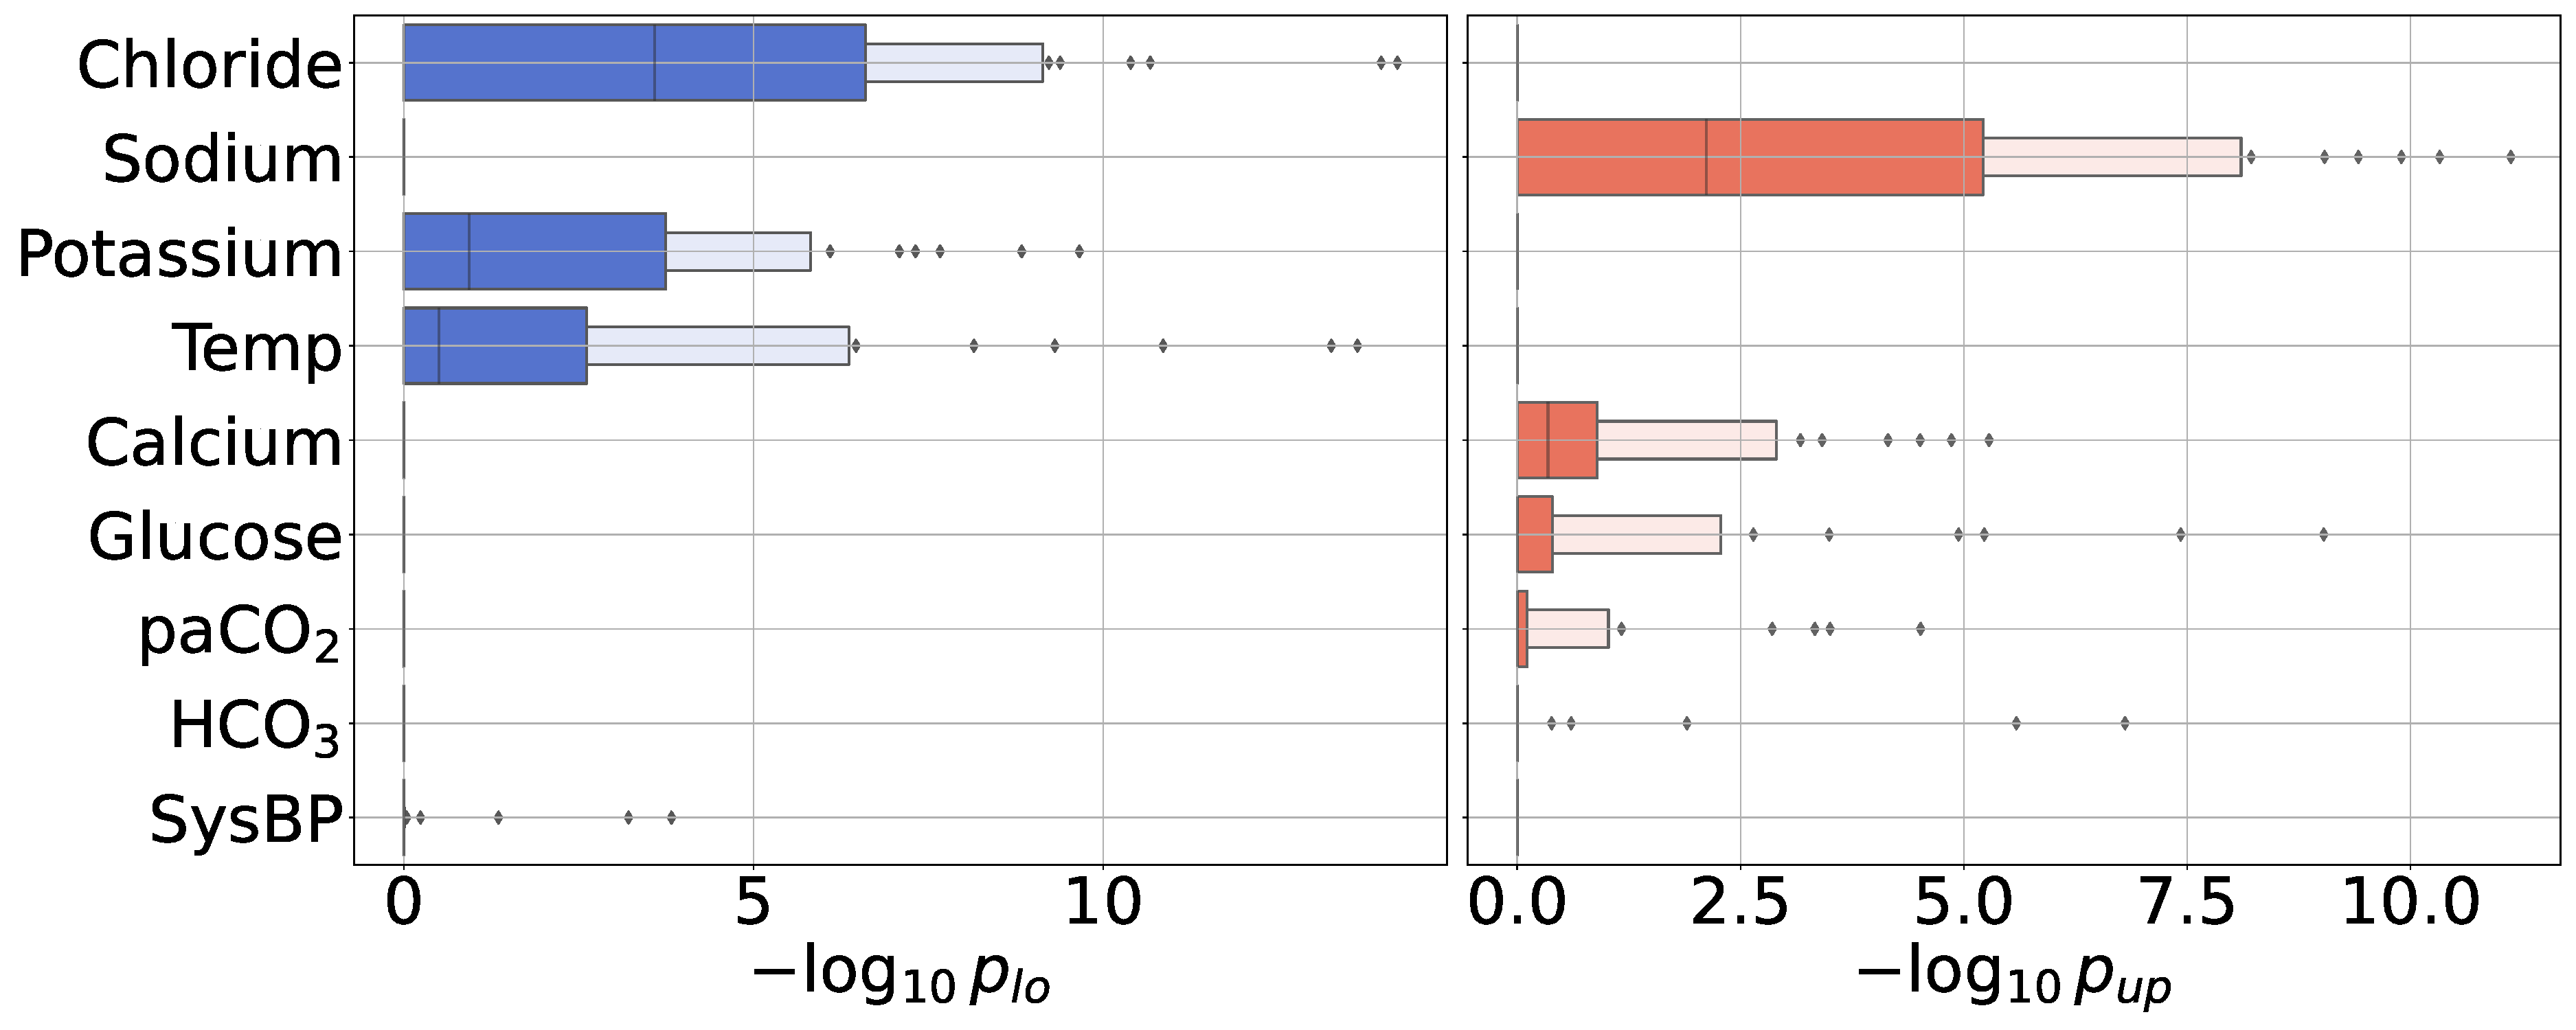
\includegraphics[height=5.5cm]{figures/causal/latest_experimental_results/p_values_nogray.pdf}
    \caption{Distributions of $-\log_{10}{p_\textup{lo}}$ and $-\log_{10}{p_\textup{up}}$ across hypotheses, grouped by physiological quantity. Higher values indicate greater evidence in favour of rejection.}
    \label{fig:p_values}
\end{figure}



\subsection{Pitfalls of naive assessment}

A naive approach to twin assessment involves simply comparing the output of the twin with observational data directly without accounting for causal considerations.
We now show that, unlike our methodology, the results produced in this way can be potentially misleading.
%
In Figure \ref{fig:longitudinal_plots}, for two different choices of $(\ax_{1:4}, \B_{1:4})$, we plot estimates of $\Qt_\tx$ and $\Q^{\textup{obs}}_\tx$ for $\tx \in \{1, \ldots, 4\}$, where
%
\begin{align*}
    \Qt_\tx &\coloneqq \E[\Yt(\ax_{1:\tx})\mid \X_0 \in \B_0, \Xt_{1:\tx}(\X_0, \ax_{1:\tx}) \in \B_{1:\tx}],\\
    \Q^{\textup{obs}}_\tx &\coloneqq \E[\Y(\A_{1:\tx})\mid \X_{0:\tx}(\A_{1:\tx})\in \B_{0:\tx}, \A_{1:\tx}=\ax_{1:\tx}]. \notag
\end{align*}

%
%
%
%
%
Here $\Qt_\tx$ is just $\Qt$ as defined above with its dependence on $\tx$ made explicit.
Each plot also shows one-sided 95\% confidence intervals on $\Qlo$ and $\Qup$ at each $\tx \in \{1, \ldots, 4\}$ obtained from Hoeffding's inequality. 
Directly comparing the estimates of $\Qt_\tx$ and $\Q^{\textup{obs}}_\tx$ would suggest that the twin is comparatively more accurate for the right-hand plot, as these estimates are closer to one another in that case.
However, the output of the twin in the right-hand plot is falsified at $\tx = 1$, as can be seen from the fact that confidence interval for $\Qt_1$ lies entirely above the one-sided confidence interval for $\Qup$ at that timestep.
On the other hand, the output of the twin in the left-hand plot is not falsified at any of the timesteps shown, so that the twin may in fact be accurate for these $(\ax_{1:4}, \B_{1:4})$, contrary to what a naive assessment strategy would suggest.
Our methodology provides a principled means for twin assessment that avoids drawing potentially misleading inferences of this kind.


A similar phenomenon appears in Figure \ref{fig:histograms}, which for two choices of $\B_{0:\tx}$ and $\ax_{1:\tx}$ shows histograms of raw glucose values obtained from the observational data conditional on $\A_{1:\tx}=\ax_{1:\tx}$ and $\X_{0:\tx}(\A_{1:\tx})\in \B_{0:\tx}$, and from the twin conditional on $\Xt_{0:\tx}(\ax_{1:\tx})\in \B_{0:\tx}$.
(Note that these raw values differ slightly from $\Y(\A_{1:\tx})$ and $\Yt(\ax_{1:\tx})$ since they are not clipped to lie between $\ylo$ and $\yup$.)
%
Below each histogram we also show 95\% confidence intervals for $\Qup$ and $\Qt$ obtained from Hoeffding's inequality.
While Figures \ref{fig:glucosea} and \ref{fig:glucoseb} appear visually very similar, the inferences produced by our testing procedure are different: the hypothesis corresponding to the right-hand plot is rejected, since there is no overlap between the confidence intervals underneath, while the hypothesis corresponding to the left-hand plot is not.
This was not an isolated case and several other examples of this phenomenon are shown in Figure \ref{fig:histograms-supplement} in the \AppendixName. 
This demonstrates that our methodology does not simply rely on direct comparison of observed and simulated trajectories, but also accounts for the possibility of confounding in the data.

%
%
%
%
%



\begin{figure}%
    \centering
    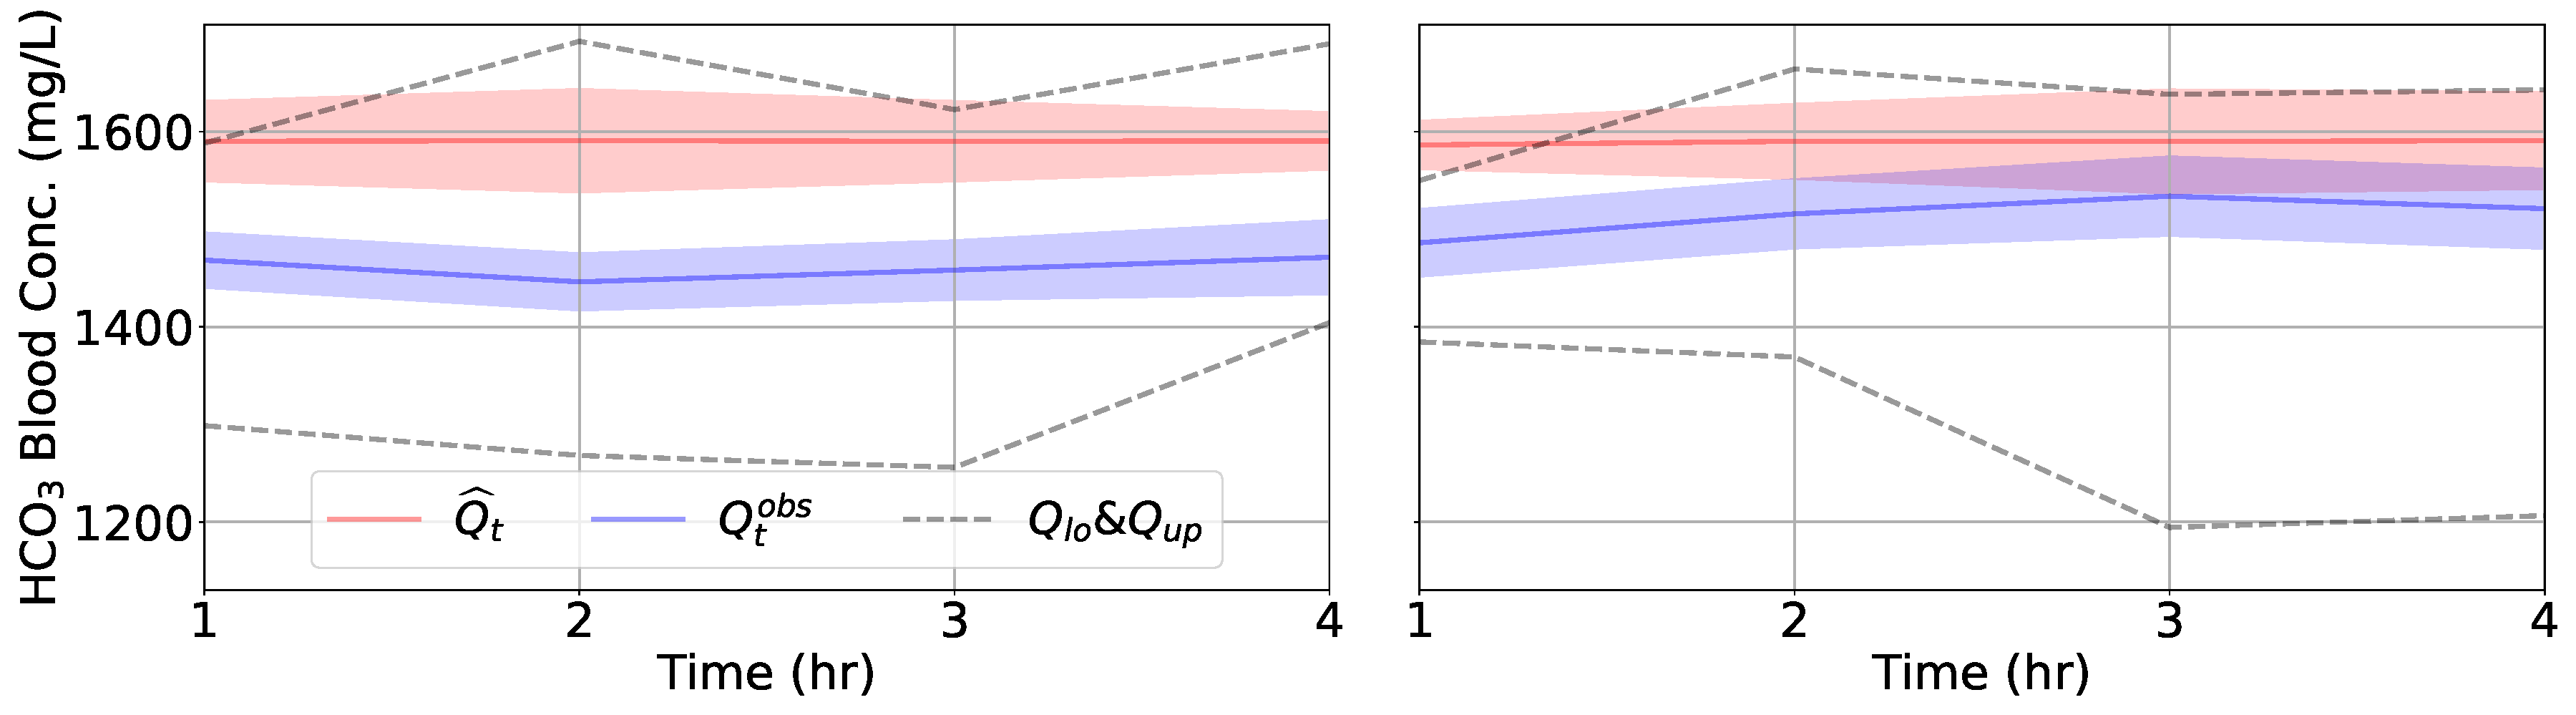
\includegraphics[height=4.5cm]{figures/causal/longitudinal_plots/HCO3_hyp_38v37_longitudinal_nogray.pdf}
    \caption{Estimates and 95\% confidence intervals for $\Qt_\tx$ and $\Q^{\textup{obs}}_\tx$ at each $1\leq \tx \leq 4$ for two choices of $(\B_{0:4}, \ax_{1:4})$, where $\Yt(\ax_{1:\tx})$ and $\Y(\ax_{1:\tx})$ correspond to HCO$_3$ blood concentration.
    The dashed lines indicate lower and upper 95\% confidence intervals for $\Qlo, \Qup$ respectively.  }
    \label{fig:longitudinal_plots}
\end{figure}

\begin{figure}%
    \centering
    \begin{subfigure}[b]{0.5\textwidth}
    \centering
    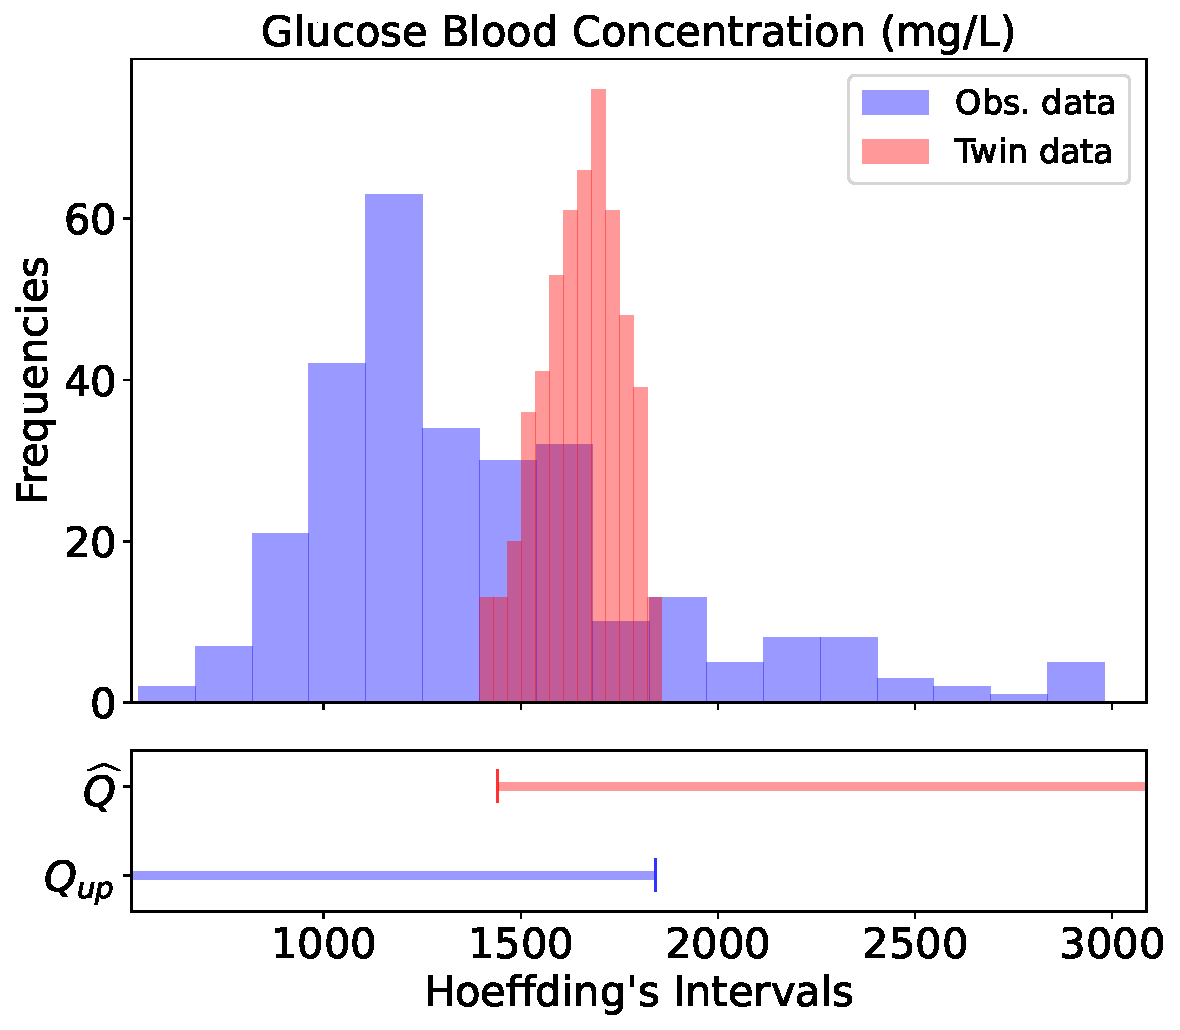
\includegraphics[height=6cm]{figures/causal/latest_experimental_results/truncated_hists/Glucose_hyp_1_with_hoeff_onesided_loFalse_p0.2_nogray.pdf}
    \subcaption{Not rejected}
    \label{fig:glucosea}
    \end{subfigure}%
    \begin{subfigure}[b]{0.5\textwidth}
    \centering
    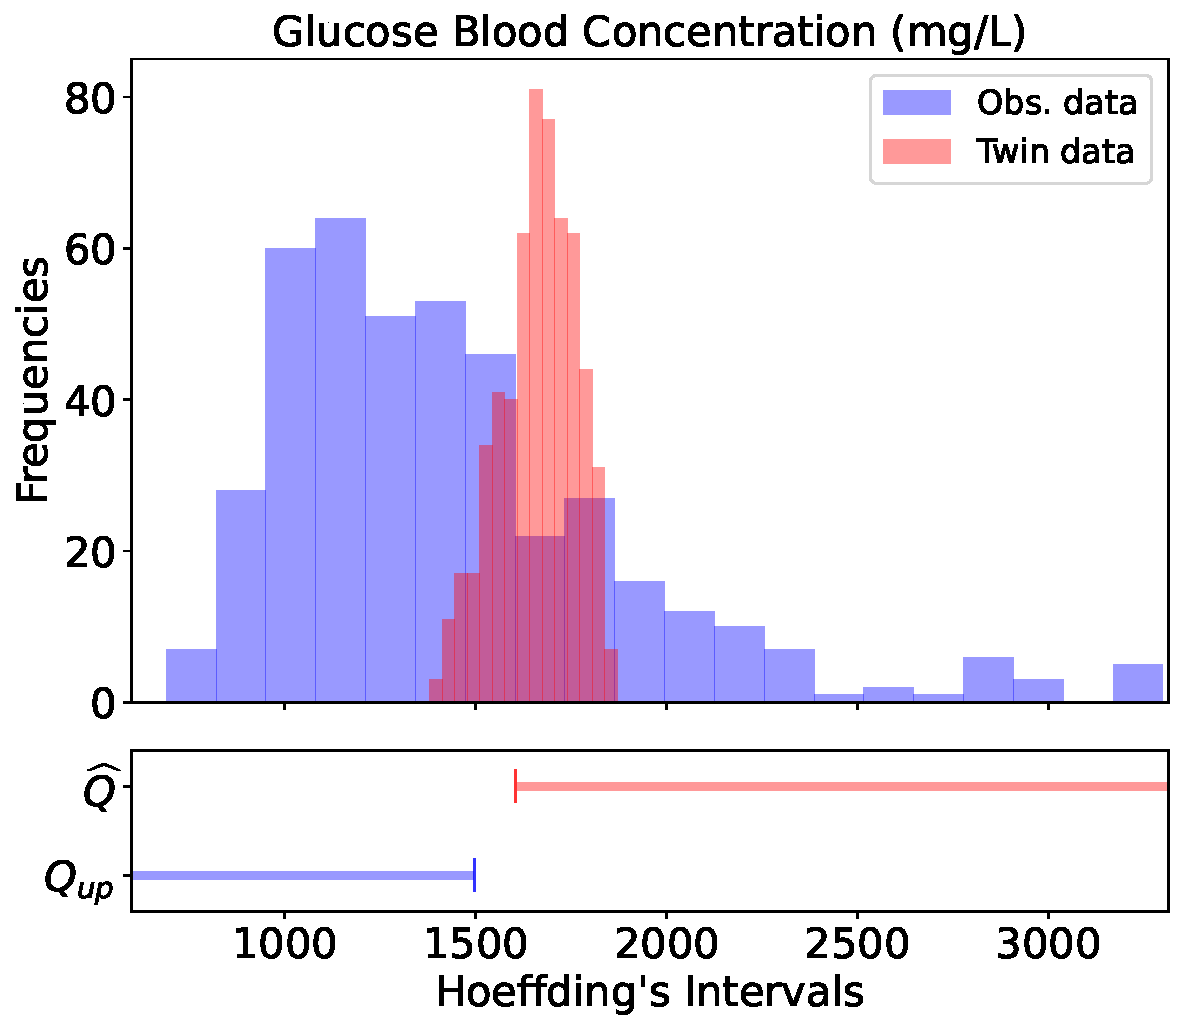
\includegraphics[height=6cm]{figures/causal/latest_experimental_results/truncated_hists/Glucose_hyp_5_with_hoeff_onesided_loFalse_p0.2_nogray.pdf}
    \subcaption{Rejected}
    \label{fig:glucoseb}
    \end{subfigure}
    %
    %
    %
    %
    %
    %
    %
    %
    %
    %
    \caption{Raw glucose values from the observational data and twin for two choices of $(\B_{0:\tx}, \ax_{1:\tx})$, with confidence intervals for $\Qt$ and $\Qup$ shown below. The horizontal axes are truncated to the .025 and .975 quantiles of the observational data for clarity. Untruncated plots are shown in Figure \ref{fig:histograms-supplement} of the \AppendixName.}
    %
    %
        %
    \label{fig:histograms}
\end{figure}


\section{Discussion}

We have advocated for a causal approach to digital twin assessment, and have presented a statistical procedure for doing so that obtains rigorous theoretical guarantees under minimal assumptions.
We now highlight the key limitations of our approach.
Importantly, our methodology implicitly assumes that the interventional distribution of the real-world process does not differ between when our dataset was obtained and when the twin is deployed to production. %
%
If the conditional distribution of $\X_{1:\T}(\ax_{1:\T})$ given $\X_0$ changes at deployment time, then so too does the set of twins that are interventionally correct, and if this change is significant enough, our assessment procedure may yield misleading results.
%
%
%
%
%
%
Distribution shift in this sense is a separate issue to unobserved confounding, and arises in a wide variety of statistical problems beyond ours.

Additionally, the procedure we used in our case study to choose the hypothesis parameters $\B_{0:\tx}$ was ad hoc.
For scalability, it would likely be necessary to obtain $\B_{0:\tx}$ via a more automated procedure.
It may also be desirable to choose $\B_{0:\tx}$ dynamically in light of previous hypotheses tested, zooming in to regions containing possible failure modes to obtain increasingly granular information about the twin.
We see opportunities here for using machine learning techniques, but leave this to future work.

%


%
%


%
%
%
%

Various other extensions and improvements appear possible.
For example, it is possible to replace our one-sided confidence intervals for $\Qlo$, $\Qup$, and $\Qt$ with two-sided ones, and thereby to obtain a procedure that may yield more precise information about the twin than we obtain by rejecting one of $\Hlo$ or $\Hup$.
We outline this at a high level in Section \ref{sec:two-sided-intervals-supplement} of the \AppendixName.
It also seems possible to leverage ideas from the literature on partial identification \cite{manski2003partial} to obtain greater statistical efficiency, for example by building on the line of work initiated by \cite{imbens2004confidence} for obtaining more informative confidence intervals.
%
%
Beyond this, it may be useful in some contexts to consider additional assumptions that lead to less conservative assessment results.
For example, various methods for \emph{sensitivity analysis} have been proposed that model the \emph{degree} to which the actions of the behavioural agent are confounded \cite{rosenbaum2002observational,tan2006distributional,yadlowsky2022bounds}.
This can yield tighter bounds on $\Q$ than are implied by Theorem \ref{thm:causal-bounds}, albeit at the expense of less robustness if these assumptions are violated.


%
%
%
%
%
%
%
%
%

%